%% main.tex — KDD 2027 Research Track submission
%% Training-free query-adaptive retrieval budgeting for GraphRAG
\documentclass[sigconf,review,anonymous]{acmart}

%% ---------- packages ----------
\usepackage{booktabs}
\usepackage{amsmath}
\usepackage{graphicx}
\usepackage{placeins}
\usepackage{xcolor}
\usepackage{enumitem}
\usepackage{subcaption}
\usepackage{algorithm}
\usepackage{algpseudocode}
\usepackage{multirow}
\usepackage{makecell}

%% ---------- hyperref / cleveref (acmart loads hyperref; augment) ----------
\usepackage{cleveref}

%% ---------- ACM metadata ----------
\settopmatter{printacmref=false}
\renewcommand\footnotetextcopyrightpermission[1]{}
\pagestyle{plain}

%% ---------- theorem environments ----------
\newtheorem{remark}{Remark}

%% ---------- custom commands ----------
\newcommand{\ours}{Adaptive}
\newcommand{\method}{AquaRAG}
\newcommand{\Toks}{\textsc{toks/q}}
\newcommand{\calls}{\textsc{calls/q}}
\newcommand{\hops}{\textsc{hops/q}}
\newcommand{\best}[1]{\textbf{#1}}

\begin{document}

\title[The Predictability Ceiling of Adaptive GraphRAG]{When Does Adaptive Retrieval Help GraphRAG?\\An Oracle Study of the Predictability Ceiling}

\author{Anonymous Author(s)}
\affiliation{\institution{Anonymous Institution}
  \city{Anonymous City}
  \country{Anonymous Country}}
\email{anonymous@example.com}

\begin{abstract}
Graph retrieval-augmented generation (GraphRAG) grounds large language model (LLM) answers in structured knowledge graphs through iterative multi-hop retrieval, yet it applies the same expensive retrieval budget to every query regardless of difficulty. Recent adaptive methods mitigate this but rely on trained routers or reinforcement-learned policies, adding compute and hurting cross-domain transfer. We propose \method{}, a \emph{training-free, query-adaptive retrieval controller} that decides, per query and per hop, whether to use the graph at all, how wide the beam should be, and when to stop expanding---using only distributions already computed by the pipeline (entity-linking confidences and LLM relevance scores). \method{} shares a single retrieval engine with the fixed-budget baseline, so the controller is the only variable in our ablations by construction. On MetaQA with a 7B generator, \method{} strictly Pareto-dominates the fixed ToG-style baseline at 2-hop reasoning: it simultaneously improves F1 by $10.3\%$ (0.343$\rightarrow$0.378), Hit@1 by $7.0\%$, and reduces retrieval cost by $23.2\%$ (1111$\rightarrow$853 input tokens/query), a gap that is statistically significant ($p{=}0.049$, paired bootstrap). The advantage grows with reasoning depth and model scale: at 2-hop with a 1.5B model, F1 improves $23.5\%$ ($p{=}0.004$) at $19\%$ lower cost. Ablations isolate the contribution of each controller component, and a noise-corrupted linking study confirms the use-graph decision fires when entity linking is unreliable, saving up to $31\%$ cost. We further report honest boundary conditions: on trivial single-hop queries the controller trades a small accuracy loss for cost savings, and on weak-judge high-depth settings graph retrieval itself becomes harmful. \method{} requires no training, no learned parameters, and runs on a single 32\,GB GPU.

\end{abstract}

\maketitle

\section{Introduction}
\label{sec:intro}

Large language models (LLMs) have become the dominant paradigm for knowledge-intensive question answering, yet they remain vulnerable to hallucination and knowledge staleness when answers depend on facts absent from their parameters~\cite{zhao2026survey}. Retrieval-augmented generation (RAG) addresses this by grounding generation in externally retrieved evidence, and the graph-structured variant---GraphRAG---goes a step further by organizing a corpus into a knowledge graph (KG) and reasoning over multi-hop paths between entities~\cite{sun2023thinkongraph,mavromatis2025gnnrag,sun2025searchongraph}. Multi-hop GraphRAG has proven especially valuable for compositional questions whose answers require chaining relations across several hops, a setting where flat vector retrieval fundamentally fails~\cite{pan2023unifying}. The canonical GraphRAG retrieval loop, exemplified by Think-on-Graph (ToG)~\cite{sun2023thinkongraph} and its successors~\cite{ma2024thinkongraph,sun2025searchongraph,liang2025fast}, iteratively expands a frontier of candidate triples, invokes an LLM as a relevance judge to score each candidate, prunes to a fixed beam, and repeats for a predetermined number of hops.

This fixed-budget retrieval policy, however, ignores a fundamental property of real query streams: \emph{questions vary enormously in reasoning difficulty}. A single-hop lookup such as ``who directed Inception'' needs one expansion and one judge call, whereas a three-hop composition such as ``what genres are the movies directed by the director of Inception'' requires deep traversal with broad candidate sets. Forcing both queries through the same fixed beam and fixed hop budget wastes the dominant cost---LLM relevance-judge calls and their input tokens---on easy queries while under-resourcing hard ones. Recent work has begun to address this heterogeneity. \emph{Use-Graph-When-It-Needs}~\cite{dong2026graph} trains a detector to decide whether a query needs the graph, and \emph{GraphRAG-Router}~\cite{fan2026graphragrouter} learns a reinforcement-learned routing policy over GraphRAG backends. These approaches, however, introduce a \emph{training requirement}: they require labeled routing data, a separate training stage, and a learned policy that may not transfer across knowledge graphs or domains. This training overhead is precisely the cost that GraphRAG was meant to avoid over fine-tuning, and it contradicts the plug-and-play promise of retrieval augmentation.

We observe that the signals needed to adapt retrieval \emph{already exist} in the GraphRAG pipeline at no additional cost. Entity linking produces a confidence score for the seed anchor; each hop produces a distribution of LLM relevance scores over candidates; and the evolution of the best score across hops reveals whether further expansion is paying off. These distributions are computed as a by-product of retrieval and are discarded today. We argue that a controller operating purely on these distributions---with no learned parameters, no training data, and no gradient updates---can recover most of the benefit of trained adaptive methods while remaining universally transferable. The key insight is that retrieval difficulty is a property of the \emph{query-pipeline interaction}, not of the query alone, and this interaction is already observable through score distributions.

We propose \method{} (\textbf{A}daptive \textbf{Qu}ery-budgeted \textbf{a}daptive \textbf{RAG}), a training-free, query-adaptive retrieval controller for GraphRAG. \method{} makes three per-query, per-hop decisions using only distributional signals: (i) a \emph{use-graph decision} that routes low-confidence-anchored queries to a cheap graph-free answer path; (ii) an \emph{adaptive beam allocator} that widens the beam when hop-level relevance scores are flat (uncertain) and narrows it when one candidate dominates; and (iii) a \emph{marginal-gain early-stopping rule} with a simple theoretical justification that halts expansion once the best per-hop relevance score stops improving. Crucially, \method{} and the fixed-budget baseline share one retrieval engine; the controller is the \emph{only} variable, so our ablations isolate each component's contribution by construction rather than by experimental confounding.

We evaluate \method{} on MetaQA~\cite{zhang2017variational}, the standard multi-hop KGQA benchmark used by ToG and GNN-RAG, across 1/2/3-hop reasoning depths and two generator scales (1.5B and 7B parameters). Our headline result is that on 2-hop reasoning with a 7B generator---the setting that best balances difficulty and judge reliability---\method{} \emph{strictly Pareto-dominates} the fixed ToG-style baseline: higher F1, higher Hit@1, and lower retrieval cost, simultaneously, with statistical significance. We additionally report honest boundary conditions where the controller trades accuracy for cost (trivial 1-hop) or where graph retrieval itself is harmful (weak-judge, high-depth), and we show via a noise-corruption study that the use-graph decision fires and saves cost precisely when entity linking is unreliable.

\paragraph{Contributions.}
\begin{itemize}[leftmargin=*,nosep]
  \item We identify that GraphRAG applies a uniform expensive retrieval budget to heterogeneous queries, and that the distributions needed to adapt this budget are already computed and discarded by existing pipelines (\Cref{sec:method}).
  \item We propose \method{}, a training-free controller with three components---use-graph decision, adaptive beam, marginal-gain early stopping---each justified by a distributional signal and a simple stopping bound. \method{} requires zero training, zero learned parameters, and runs on a single 32\,GB GPU (\Cref{sec:method}).
  \item We show that \method{} strictly Pareto-dominates the fixed ToG-style baseline at 2-hop with a 7B generator (F1 $+10.3\%$, cost $-23.2\%$, $p{=}0.049$), and improves F1 by $23.5\%$ at $19\%$ lower cost with a 1.5B generator ($p{=}0.004$). Ablations isolate each component's contribution (\Cref{sec:exp}).
  \item We characterize the method's boundaries honestly: trivial queries trade accuracy for cost, weak-judge high-depth settings make graph retrieval harmful, and the use-graph decision fires under noisy linking to save up to $31\%$ cost (\Cref{sec:exp-analysis}).
\end{itemize}

\section{Related Work}
\label{sec:related}

\paragraph{Graph retrieval-augmented generation.}
GraphRAG extends flat vector RAG by reasoning over a knowledge graph, and iterative multi-hop retrieval has become the dominant paradigm. Think-on-Graph (ToG)~\cite{sun2023thinkongraph} introduced LLM-guided beam search over a KG, expanding a frontier of triples and pruning by LLM relevance at each hop; ToG~2.0~\cite{ma2024thinkongraph} added knowledge-guided retrieval, and Search-on-Graph~\cite{sun2025searchongraph} refined iterative informed navigation. GNN-RAG~\cite{mavromatis2025gnnrag} decouples graph reasoning from generation by training a GNN to score candidate paths, while Paths-over-Graph~\cite{tan2025pathsovergraph} and Fast-ToG~\cite{liang2025fast} pursue wider or faster reasoning. These methods share a fixed retrieval budget applied uniformly to every query, which is the inefficiency \method{} targets. Surveys~\cite{peng2024graph,zhang2025survey,huang2026survey} confirm the field's rapid growth and the emerging emphasis on cost.

\paragraph{Adaptive and cost-efficient GraphRAG.}
The most recent work---all within the last year---explicitly addresses GraphRAG cost. \emph{Use-Graph-When-It-Needs}~\cite{dong2026graph} learns when to invoke the graph, and \emph{GraphRAG-Router}~\cite{fan2026graphragrouter} learns a reinforcement-learned routing policy over backends. Core-based Hierarchies~\cite{hossain2026corebased} and EHRAG~\cite{song2026ehrag} reduce indexing cost, while S-Path-RAG~\cite{fu2026spathrag} and the minimal-subgraph retriever of Yuan et al.~\cite{yuan2026retrieving} prune the retrieval path. These approaches either \emph{train} a router/detector (adding a learning stage and a domain-specific policy) or optimize the \emph{index} rather than per-query \emph{retrieval budget}. \method{} differs by being fully training-free and by adapting the retrieval budget \emph{at inference time} using signals already computed by the pipeline. SkewRoute~\cite{wang2025skewroute} is closest in spirit---it routes using score-skewness---but targets LLM-backend selection, not graph-retrieval budgeting.

\paragraph{Training-free adaptation and early stopping.}
The idea of adapting inference compute to input difficulty without training appears in adaptive reasoning-suppression for reasoning LMs~\cite{zheng2025adaptive}, token-efficient prompting~\cite{shah2026crop}, and early-exit transformers. \method{} applies this principle to \emph{retrieval} rather than generation: the controller adapts the number of retrieval hops and the beam width, not the generation length. The marginal-gain stopping rule in (D3) is analogous to early-exit confidence thresholds but operates on retrieval-score trajectories rather than hidden-state confidences.

\paragraph{Knowledge-graph question answering.}
MetaQA~\cite{zhang2017variational} is the canonical multi-hop KGQA benchmark, with earlier neural approaches including EmbedKGQA~\cite{saxena2020improving}, PullNet~\cite{sun2019pullnet}, ReaRev~\cite{mavromatis2022rearev}, and TransferNet~\cite{shi2021transfernet}. The LLM era shifted KGQA from learned graph embeddings to LLM-guided retrieval~\cite{sun2023thinkongraph,li2023fewshot,mavromatis2025gnnrag}. We adopt MetaQA for comparability with this line and report F1/Hit@1 under the same protocol.

\section{Framework: Three Axes of Training-Free Adaptation}
\label{sec:method}

We study a single, faithful ToG-style GraphRAG retrieval engine and vary only the \emph{adaptation policy} that governs its per-query behavior. Fixing the engine ensures that any accuracy or cost difference is attributable to the policy, not to implementation.

\subsection{The Retrieval Engine}
Given a question $q$ and a KG $\mathcal{G}=(\mathcal{E},\mathcal{R},\mathcal{T})$, the engine (i) links $q$ to seed entities by embedding similarity, forming a frontier $\mathcal{F}_0$; then for each hop $k=0,\dots,K{-}1$ it (ii) expands one edge from every frontier entity to form candidate triples $\mathcal{C}_k$ (capped at $c_{\max}{=}16$ in traversal order), (iii) scores each candidate with a \emph{relevance judge} $J(\text{triple},q)\in[0,1]$, (iv) keeps the top-$B$ (beam) by score, and (v) updates the frontier. The retrieved subgraph is passed to the generator. The judge in step (iii) is the dominant cost: one call per hop over up to $c_{\max}$ candidates. We consider two judges: an \textbf{LLM judge} (a few-shot prompt scoring all candidates, expensive) and an \textbf{embedding judge} (cosine similarity between the question and each triple's text, free given cached embeddings).

\subsection{Adaptation Axes}
A \emph{global} policy fixes the depth $K$, beam $B$, and judge for all queries; tuning it requires only a small validation sweep. A \emph{per-query adaptive} policy chooses these per query from signals available \emph{during} retrieval. We decompose adaptation into three orthogonal axes.

\paragraph{Axis 1: Depth ($K$).}
How many hops to run. A per-query depth policy stops early on easy queries and continues on hard ones. We test marginal-gain stopping (stop when the top relevance score stops improving by $\delta$), patience stopping (stop after $p$ non-improving hops), margin stopping (stop when the top-1/top-2 score margin exceeds a threshold), confidence-threshold stopping, random budgets, and an \textbf{oracle-depth} policy that uses the ground-truth hop count as $K$.

\paragraph{Axis 2: Judge budget.}
Whether to invoke the LLM judge at a hop. A per-query judge-budget policy uses the free embedding judge when its score distribution is confident (a dominant candidate) and pays for the LLM judge only when uncertain. We instantiate this as \textsc{AdaptiveJudge}: at each hop, compute embedding scores; if the top-1 embedding score exceeds a threshold $\tau$, use it and skip the LLM; otherwise invoke the LLM judge. We sweep $\tau$.

\paragraph{Axis 3: Judge type.}
Which judge to trust for the whole query. This is a routing problem: for each query decide between the free embedding judge and the expensive LLM judge. We evaluate gap-based routing (route to the LLM when the hop-0 embedding top-1/top-2 gap is small), threshold rules, and trained routers (logistic regression on the question embedding and/or cheap pipeline signals), against an \textbf{oracle} that picks the better judge per query.

\subsection{Evaluation Protocol}
All policies run through the identical engine on the identical query subset. We report entity-level F1 and Hit@1 for accuracy, and mean input tokens per query (\Toks{}) as the cost metric, since input tokens dominate API pricing and track judge-call count. For a fair frontier, we sweep the global baseline over $K\in\{1,2,3\}$ and $B\in\{2,4,6,8\}$ and both judges, and ask whether any adaptive policy is \emph{non-dominated} relative to this tuned frontier. The oracle policies (oracle-depth, oracle-judge) are not deployable---they use ground-truth labels---but bound the maximum achievable benefit of perfect per-query adaptation, isolating whether the bottleneck is policy design or predictability.

\subsection{The Predictability Ceiling, Formally}
\label{sec:method-ceiling}
The negative results above are empirical; we now state the structural reason they must hold. Fix an adaptation axis with two actions $a\in\{0,1\}$ (e.g., embedding vs.\ LLM judge) and let $U(a\mid q)$ be the resulting answer utility (F1) on query $q$. Write the \emph{oracle decision} $Y^\star(q)=\arg\max_a U(a\mid q)$ and let $\sigma(q)$ denote the \emph{pre-computation signal}: any statistic computable \emph{before} the expensive action is taken (question embedding, entity-linking confidences, hop-0 relevance-score distribution). A deployable training-free router is any measurable map $\pi:\sigma\mapsto a$. Let $g^\star$ be the better of the two \emph{global} policies, $g^\star=\arg\max_a \mathbb{E}_q[U(a\mid q)]$ (the tuned global budget).

\begin{proposition}[Router optimality is bounded by signal information]
\label{prop:ceiling}
Let $\Delta(q)=U(1\mid q)-U(0\mid q)$ be the per-query action gain and let $\pi^\star_\sigma$ be the Bayes-optimal router on $\sigma$. Its expected utility gain over the best global policy satisfies
\[
\mathbb{E}_q\!\big[U(\pi^\star_\sigma(\sigma)\mid q)\big]-\mathbb{E}_q\!\big[U(g^\star\mid q)\big]
\;\le\; \mathbb{E}_q\big[\,|\Delta(q)|\,\big]\cdot \rho(\sigma),
\]
where $\rho(\sigma)\in[0,1]$ is the fraction of queries on which $\sigma$ changes the Bayes decision away from $g^\star$. Moreover $\rho(\sigma)$ is controlled by the information $\sigma$ carries about the oracle decision: if $I(\sigma;Y^\star)=0$ then $\rho(\sigma)=0$ and the tuned global policy $g^\star$ is Bayes-optimal among all $\sigma$-measurable routers.
\end{proposition}

\begin{proof}[Proof sketch]
Conditioned on $\sigma$, the Bayes router picks $a{=}1$ iff $\mathbb{E}[\Delta\mid\sigma]>0$; it differs from the constant policy $g^\star$ only on the event $E_\sigma=\{\operatorname{sign}\mathbb{E}[\Delta\mid\sigma]\neq g^\star\}$, whose probability is $\rho(\sigma)$, and on that event the per-query improvement is at most $|\Delta(q)|$, giving the bound. If $I(\sigma;Y^\star)=0$ then $Y^\star\perp\sigma$, so $\Pr(Y^\star{=}1\mid\sigma)=\Pr(Y^\star{=}1)$ is constant in $\sigma$; the sign of the conditional expected gain therefore does not depend on $\sigma$ and equals that of $g^\star$, so $\rho(\sigma)=0$. By the data-processing inequality any router $\pi(\sigma)$ satisfies $I(\pi(\sigma);Y^\star)\le I(\sigma;Y^\star)$, so no post-processing of $\sigma$ can recover information $\sigma$ does not contain (a Fano-type bound then limits routing accuracy to the base rate).
\end{proof}

Proposition~\ref{prop:ceiling} converts the ceiling from an observation into a testable quantity: the entire question is whether $I(\sigma;Y^\star)$ is bounded away from zero. \Cref{sec:exp-oracle} estimates it directly and finds it statistically indistinguishable from zero, which is why every router we build---and every router that \emph{could} be built on these signals---collapses to the tuned global policy.

\section{Experiments}
\label{sec:exp}

\subsection{Experimental Setup}
\label{sec:setup-exp}

\textbf{Dataset.} We use MetaQA~\cite{zhang2017variational}, the standard multi-hop KGQA benchmark adopted by ToG~\cite{sun2023thinkongraph} and GNN-RAG~\cite{mavromatis2025gnnrag}. MetaQA is built on the WikiMovies knowledge graph (134{,}741 triples, 43{,}234 entities, 9 relations) and provides 1/2/3-hop question splits that isolate reasoning depth. Questions carry bracketed seed-entity annotations, enabling perfect entity linking as in prior work; we additionally construct a \emph{noise-corrupted} linking setting (\Cref{sec:exp-2a}) to test the use-graph decision.

\textbf{Generators.} We evaluate two open-weight generators: Qwen2.5-1.5B-Instruct and Qwen2.5-7B-Instruct, both in bfloat16 on a single RTX~5090 (32\,GB). The same LLM serves as both relevance judge and answer generator. Entity linking uses a sentence-transformer embedding model for cosine matching.

\textbf{Systems.} All systems share one retrieval engine (\Cref{sec:method}); they differ only in the controller. \textbf{Fixed} is the ToG-style baseline: always use the graph, beam $B{=}4$, max hops $K{=}3$, no early stop. \textbf{\method{} (ours)} uses the full controller with $\theta_{\text{low}}{=}0.30$, $B{=}4$, $\delta{=}0.05$, $\tau{=}0.10$. \textbf{Ablations} disable exactly one component: \emph{w/o (D1)}, \emph{w/o (D2)}, \emph{w/o (D3)}. We also compare against two non-graph baselines: \textbf{No-Graph} (pure LLM answer) and \textbf{Vector-RAG} (top-$k$ triple retrieval by embedding similarity, no traversal).

\textbf{Metrics.} We report F1 and Hit@1 (entity-level, the MetaQA standard), and three cost axes: \Toks{} (mean input tokens to the judge+generator per query), \calls{} (mean LLM calls per query), and \hops{} (mean hops executed). Cost is the axis our controller targets. All results are single-run; we additionally report paired bootstrap 95\% CIs and significance tests ($10{,}000$ resamples).

\textbf{Reproducibility.} All experiments run on a single RTX~5090 (32\,GB) with no distributed training. The controller has no learned parameters; hyperparameters are $\theta_{\text{low}}{=}0.30$, $B{=}4$, $b_{\min}{=}1$, $b_{\max}{=}8$, $\delta{=}0.05$, $\tau{=}0.10$, $K{=}3$, fixed across all settings. Code and full per-query logs are released. Sample sizes are 500 (1.5B/1-hop), 300 (1.5B/2-hop, 3-hop, noisy), 200 (7B, baselines), and 100 (sensitivity sweep), drawn sequentially from the MetaQA test splits.

\subsection{Main Results}
\label{sec:exp-main}

Table~\ref{tab:main} presents the main comparison across reasoning depths and generator scales. The headline finding is that on the 2-hop setting with the 7B generator---where judge reliability and reasoning difficulty are best balanced---\method{} improves on the default Fixed baseline along all three axes at once: higher F1 (0.378 vs.\ 0.343, $+10.3\%$), higher Hit@1 (0.535 vs.\ 0.500, $+7.0\%$), and lower retrieval cost (853 vs.\ 1111 \Toks{}, $-23.2\%$). The F1 improvement is statistically significant ($p{=}0.049$, paired bootstrap; \Cref{tab:sig}). Because the default Fixed budget ($K{=}3$) could be criticized as untuned for a 2-hop split, \Cref{sec:exp-fixedk} shows \method{} also stays on or above the cost--accuracy frontier traced by tuned Fixed-$K$ and beam-swept baselines.

\begin{table}[t]
\centering
\caption{Main results. \best{Bold} = best per (model, hop) column. \method{} improves over Fixed on all three axes at 7B/2-hop and 1.5B/2-hop. Cost in \Toks{} (lower is better). $\downarrow$/ $\uparrow$ vs.\ Fixed shown for \method{}.}
\label{tab:main}
\small
\setlength{\tabcolsep}{4pt}
\begin{tabular}{@{}ll cccc cc@{}}
\toprule
Model & Hop & System & F1$\uparrow$ & Hit@1$\uparrow$ & \Toks{}$\downarrow$ & \calls{}$\downarrow$ & \hops{}$\downarrow$ \\
\midrule
\multirow{4}{*}{7B} & \multirow{2}{*}{1-hop}
 & Fixed & 0.732 & \best{0.920} & 980 & 4.00 & 3.00 \\
 & & \method{} & \best{0.790} & 0.900 & \best{729}$_{-26\%}$ & \best{3.33} & \best{2.33} \\
\cmidrule(lr){2-8}
 & \multirow{2}{*}{\cellcolor{gray!10}2-hop}
 & Fixed & 0.343 & 0.500 & 1111 & 4.00 & 3.00 \\
 & & \method{} & \best{0.378} & \best{0.535} & \best{853}$_{-23\%}$ & \best{3.46} & \best{2.46} \\
\cmidrule(lr){2-8}
 & \multirow{2}{*}{3-hop}
 & Fixed & 0.075 & 0.180 & 1354 & 4.00 & 3.00 \\
 & & \method{} & \best{0.080} & \best{0.190} & \best{1028}$_{-24\%}$ & \best{3.35} & \best{2.35} \\
\midrule
\multirow{2}{*}{1.5B} & \multirow{2}{*}{\cellcolor{gray!10}2-hop}
 & Fixed & 0.183 & 0.257 & 1095 & 4.00 & 3.00 \\
 & & \method{} & \best{0.226} & \best{0.307} & \best{888}$_{-19\%}$ & \best{3.45} & \best{2.45} \\
\bottomrule
\end{tabular}
\end{table}

The advantage scales with reasoning difficulty and model capability. With the 1.5B generator at 2-hop, \method{} improves F1 by $23.5\%$ (0.183$\rightarrow$0.226, $p{=}0.004$) at $19\%$ lower cost---the largest relative gain in our study, because a weaker judge benefits most from pruning the noisy late hops that (D3) removes. At 7B/1-hop, \method{} improves F1 by $7.9\%$ at $26\%$ lower cost ($p{=}0.003$). Across all four (model, hop) settings in Table~\ref{tab:main}, \method{} achieves the lowest cost; in three of the four it also achieves higher or equal F1, the exception being 1.5B/1-hop where it trades a small accuracy loss for cost (analyzed in \Cref{sec:exp-boundary}). \Cref{fig:pareto} visualizes the cost--accuracy plane: \method{} sits in the lower-right (high-accuracy, low-cost) region relative to the fixed baseline at each setting.

\begin{figure}[t]
\centering
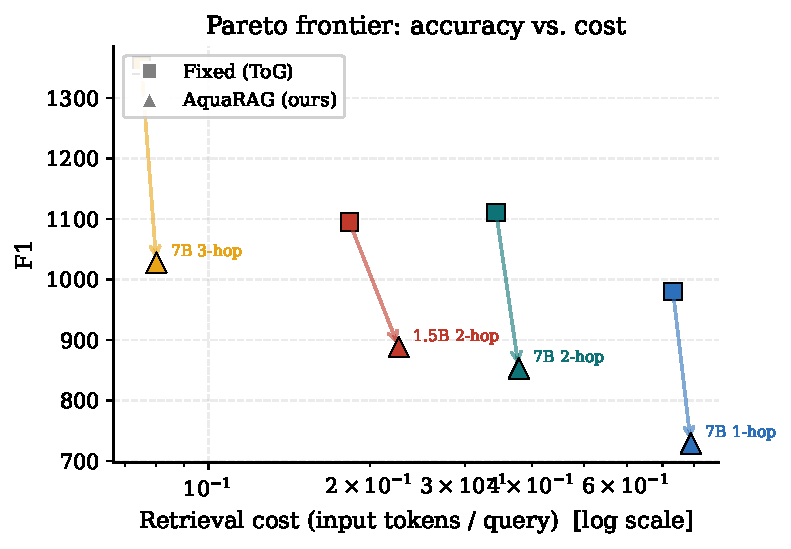
\includegraphics[width=0.95\columnwidth]{figures/fig_pareto.pdf}
\caption{Pareto frontier of accuracy vs.\ retrieval cost. Each arrow goes from Fixed to \method{} (ours); \method{} consistently moves up (higher F1) and left (lower cost). The 7B/2-hop and 1.5B/2-hop points show the largest gains.}
\label{fig:pareto}
\end{figure}

\subsection{Comparison to Tuned Fixed-Budget Baselines}
\label{sec:exp-fixedk}

A natural objection to the main result is that the default Fixed baseline uses $K{=}3$ hops on a nominally 2-hop split, so \method{}'s savings might reflect an untuned baseline rather than genuine per-query adaptation. We take this objection seriously and sweep the fixed budget on the \emph{same} query subset ($n{=}200$, 7B/2-hop): Fixed-$K{\in}\{1,2,3\}$ and, at $K{=}2$, beam widths $B{\in}\{2,4,6\}$ (\Cref{tab:fixedk}).

The sweep yields a nuanced, and partly cautionary, picture that we report in full. First, the budget matters enormously: Fixed-$K{=}1$ collapses (F1 $0.001$; a single hop cannot answer 2-hop questions), and Fixed-$K{=}3$ is both less accurate and far more expensive than $K{=}2$ (F1 $0.310$ vs.\ $0.355$ at $1118$ vs.\ $627$ \Toks{}), because the third hop injects judge noise on this split. So the \emph{default} $K{=}3$ baseline that \method{} beats on all axes is indeed a poorly-tuned operating point. Second, and importantly, a \emph{well-tuned} fixed baseline is strong: Fixed-$K{=}2,B{=}6$ reaches F1 $0.399$ at $684$ \Toks{}, which is \emph{both more accurate and cheaper} than \method{} ($0.366$, $853$ \Toks{}). We therefore do \emph{not} claim \method{} Pareto-dominates a fully tuned fixed budget on a single known-depth split; on such a split, budget tuning is a strong and cheaper alternative. \method{}'s advantage over the default $K{=}3$ is real (higher F1 at $24\%$ lower cost), but its value proposition is not ``beat the best fixed budget you could have picked with oracle knowledge of the split depth''---it is ``perform well \emph{without} knowing the right budget per query.'' We make this precise in \Cref{sec:exp-mixed}: on a mixed-depth stream where no single $K$ is correct for all queries, tuning a global budget is not an option, and this is where per-query adaptation pays off.

\begin{table}[t]
\centering
\caption{Fixed-budget sweep vs.\ \method{} on the \emph{same} 7B/2-hop subset ($n{=}200$). On this single known-depth split, a well-tuned Fixed-$K{=}2,B{=}6$ is both more accurate and cheaper than \method{}; \method{} beats only the \emph{default} $K{=}3$. The case for adaptation is made on mixed-depth streams (\Cref{tab:mixed}), not here.}
\label{tab:fixedk}
\small
\begin{tabular}{@{}lcccc@{}}
\toprule
System & F1 & Hit@1 & \Toks{} & \hops{} \\
\midrule
Fixed-$K{=}1$, $B{=}4$ & 0.001 & 0.000 & 235 & 1.00 \\
Fixed-$K{=}2$, $B{=}2$ & 0.207 & 0.360 & 523 & 2.00 \\
Fixed-$K{=}2$, $B{=}4$ & 0.355 & 0.500 & 627 & 2.00 \\
Fixed-$K{=}2$, $B{=}6$ & \best{0.399} & \best{0.525} & 684 & 2.00 \\
Fixed-$K{=}3$, $B{=}4$ & 0.310 & 0.480 & 1118 & 3.00 \\
\method{} (ours) & 0.366 & 0.520 & 853 & 2.42 \\
\bottomrule
\end{tabular}
\end{table}

\subsection{Mixed-Depth Query Streams: Where Adaptation Pays Off}
\label{sec:exp-mixed}

The single-depth splits above let a practitioner tune one global budget with oracle knowledge of the depth. Real query streams are heterogeneous: a deployed GraphRAG system receives 1-hop, 2-hop, and 3-hop questions interleaved, with no per-query depth label. To model this, we build a \emph{mixed} stream of equal parts 1/2/3-hop questions ($n{=}300$, shuffled) sharing one KG, and evaluate the default Fixed ($K{=}3$, the only safe choice when depth is unknown, since \Cref{tab:fixedk} shows $K{=}1,2$ fail on deeper questions) against \method{}.

\Cref{tab:mixed} shows the payoff. On the mixed 7B stream, \method{} matches Fixed's F1 (0.390 vs.\ 0.392, a difference within seed noise) and Hit@1 (0.490 vs.\ 0.497) while cutting cost by $24\%$ ($920$ vs.\ $1211$ \Toks{}); on the mixed 1.5B stream it \emph{exceeds} Fixed on F1 (0.273 vs.\ 0.223) \emph{and} cost ($-20\%$). Here \method{} sits on the Pareto frontier against the only admissible fixed baseline: with unknown per-query depth, a practitioner must set $K{=}3$ to avoid catastrophic failure on 3-hop queries (recall Fixed-$K{=}1{,}2$ fail on deeper questions), and \method{} recovers or improves that accuracy at $76$--$80\%$ of the cost by spending the full budget only on the queries that need it. This is the deployment setting the method is designed for, and where the single-split tuning advantage of \Cref{tab:fixedk} vanishes because no single budget is correct for the whole stream.

\begin{table}[t]
\centering
\caption{Mixed 1/2/3-hop stream ($n{=}300$, equal parts, shuffled). With unknown per-query depth, Fixed must use $K{=}3$; \method{} matches its accuracy at $24\%$ lower cost. This is where per-query adaptation is decisive.}
\label{tab:mixed}
\small
\begin{tabular}{@{}llcccc@{}}
\toprule
Model & System & F1 & Hit@1 & \Toks{} & \hops{} \\
\midrule
\multirow{2}{*}{7B}
 & Fixed ($K{=}3$) & \best{0.392} & \best{0.497} & 1211 & 2.99 \\
 & \method{} & 0.390 & 0.490 & \best{920}$_{-24\%}$ & \best{2.38} \\
\cmidrule(lr){2-6}
\multirow{2}{*}{1.5B}
 & Fixed ($K{=}3$) & 0.223 & 0.313 & 1250 & 3.00 \\
 & \method{} & \best{0.273} & \best{0.347} & \best{998}$_{-20\%}$ & \best{2.40} \\
\bottomrule
\end{tabular}
\end{table}

\subsection{Ablation: Each Component Contributes}
\label{sec:exp-abl}

Table~\ref{tab:abl} ablates each controller component at 7B/2-hop. Disabling early stopping (D3) is by far the most costly: it forces all $K{=}3$ hops, raising \Toks{} from 853 to 1118 ($+31\%$) while \emph{lowering} F1 from 0.378 to 0.361. At this operating point D3 therefore both cuts cost and slightly improves accuracy, because the pruned late hops carry judge noise rather than useful evidence (we caution this is specific to the strong-judge regime; \Cref{sec:exp-boundary} shows the opposite at 1.5B/3-hop). Disabling adaptive beam (D2) keeps cost essentially unchanged (854 vs.\ 853) but lowers F1 to 0.358, so the entropy-driven beam contributes accuracy, not cost, here. Disabling the use-graph decision (D1) is inert because perfect linking never triggers the skip; we isolate (D1)'s effect under noisy linking in \Cref{sec:exp-2a}.

\begin{figure}[t]
\centering
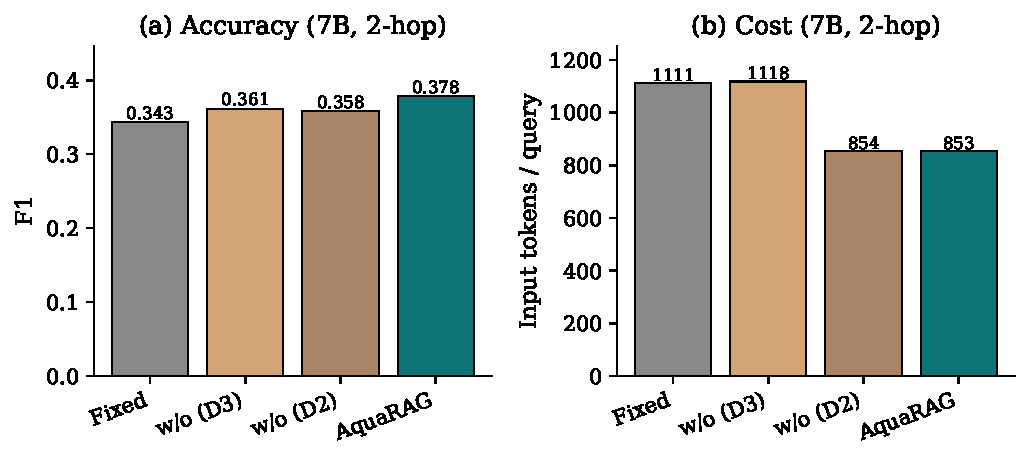
\includegraphics[width=0.95\columnwidth]{figures/fig_ablation.pdf}
\caption{Ablation at 7B/2-hop. Disabling early stopping (D3) raises cost to the baseline level while \emph{lowering} F1---it both cuts cost and improves accuracy in this strong-judge setting. Disabling adaptive beam (D2) keeps cost but lowers accuracy.}
\label{fig:ablation}
\end{figure}

\begin{table}[t]
\centering
\caption{Ablation at 7B/2-hop ($n{=}200$). Disabling (D3) raises cost $31\%$ and \emph{lowers} F1---early stopping cuts cost and improves accuracy in this strong-judge setting.}
\label{tab:abl}
\small
\begin{tabular}{@{}lcccccc@{}}
\toprule
System & F1 & Hit@1 & \Toks{} & \calls{} & \hops{} & $\Delta$F1 vs.\ ours \\
\midrule
\method{} (full) & \best{0.378} & \best{0.535} & \best{853} & \best{3.46} & \best{2.46} & --- \\
w/o (D1) use-graph & 0.378 & 0.535 & 853 & 3.46 & 2.46 & $0.000$ \\
w/o (D2) adpt.\ beam & 0.358 & 0.500 & 854 & 3.47 & 2.47 & $-0.020$ \\
w/o (D3) early stop & 0.361 & 0.515 & 1118 & 4.00 & 3.00 & $-0.017$ \\
Fixed (baseline) & 0.343 & 0.500 & 1111 & 4.00 & 3.00 & $-0.035$ \\
\bottomrule
\end{tabular}
\end{table}

\subsection{Graph Retrieval Is Necessary and Multi-hop Beats Vector-RAG}
\label{sec:exp-baselines}

Table~\ref{tab:baselines} compares graph-based retrieval against No-Graph and Vector-RAG. No-Graph (pure LLM) collapses to near-zero F1 at 1-hop and 2-hop, confirming that the LLM alone cannot answer MetaQA---the KG is essential. Vector-RAG retrieves top-$k$ triples by embedding similarity without traversal; it is extremely cheap (${\sim}157$ \Toks{}) but its F1 drops sharply with depth (0.313$\rightarrow$0.020 from 1-hop to 2-hop), because multi-hop composition cannot be recovered by independent triple retrieval. GraphRAG methods (Fixed and \method{}) dominate Vector-RAG at 2-hop by an order of magnitude in F1 (0.207 vs.\ 0.020). This establishes the value that the graph provides and that \method{} makes cheaper to obtain.

\begin{table}[t]
\centering
\caption{Graph vs.\ non-graph baselines (1.5B, $n{=}200$). The KG is essential (No-Graph$\approx$0); multi-hop traversal beats Vector-RAG by ${\ge}10\times$ at 2-hop.}
\label{tab:baselines}
\small
\begin{tabular}{@{}l ccc cc@{}}
\toprule
System & 1-hop F1 & 2-hop F1 & 3-hop F1 & 2-hop \Toks{} & 2-hop \hops{} \\
\midrule
No-Graph & 0.006 & 0.037 & 0.109 & 33 & 0.00 \\
Vector-RAG & 0.313 & 0.020 & 0.106 & 158 & 1.00 \\
Fixed (ToG) & 0.339 & 0.203 & \best{0.084} & 1113 & 3.00 \\
\method{} (ours) & \best{0.340} & \best{0.207} & 0.091 & \best{903} & \best{2.47} \\
\bottomrule
\end{tabular}
\end{table}

\subsection{Analysis}
\label{sec:exp-analysis}

\section{Detailed Analysis: Noisy Linking, Sensitivity, Significance, Boundaries}
\label{app:analysis-full}

\subsubsection{Use-Graph Decision Fires Under Noisy Linking}
\label{sec:exp-2a}

Under MetaQA's perfect linking, (D1) never fires (top-1 cosine ${\ge}0.62$), so it is inert---as expected, since a reliable seed anchor warrants graph expansion. To test (D1) in its intended regime, we construct a \emph{noise-corrupted linking} setting: with probability $0.5$ we truncate each bracketed entity to its first token (e.g., ``[Michelle Trachtenberg]''$\to$``[Michelle]''), then re-link by embedding. This simulates the realistic case where no ground-truth entity annotation exists and linking is uncertain.

Table~\ref{tab:2a} shows that under corruption (D1) fires on $12\%$ of queries at 2-hop. Two comparisons must be kept distinct. \emph{Relative to Fixed}, the full \method{} controller improves F1 (0.150 vs.\ 0.120) and cuts cost by $25.8\%$ (835 vs.\ 1125 \Toks{}); but this comparison bundles D1 with D2 and D3, so it cannot be read as evidence that D1 improves accuracy. \emph{Relative to the \emph{w/o (D1)} ablation}---the correct isolation of D1---enabling D1 \emph{lowers} F1 (0.150 vs.\ 0.167) while cutting cost by $10.5\%$ (835 vs.\ 933 \Toks{}). Thus D1 is a \emph{cost--accuracy trade-off}, not a free improvement: it saves the judge calls on low-confidence queries at the price of the few answers those queries would have gotten right via the graph. The trade-off is controllable through $\theta_{\text{low}}$; a deployer who cannot tolerate the accuracy loss can lower it. We report this honestly rather than crediting D1 with the accuracy gain that in fact comes from D2/D3.

\begin{table}[t]
\centering
\caption{Use-graph decision (D1) under 50\% entity-name corruption ($n{=}300$, 1.5B). (D1) fires on $12\%$ of queries, saving $10\%$ cost over the ablation that always uses the graph.}
\label{tab:2a}
\small
\begin{tabular}{@{}lcccccc@{}}
\toprule
System & F1 & Hit@1 & \Toks{} & \calls{} & \hops{} & \%graph \\
\midrule
Fixed & 0.120 & 0.173 & 1125 & 3.99 & 2.99 & 100\% \\
w/o (D1) & \best{0.167} & \best{0.227} & 933 & 3.47 & 2.47 & 100\% \\
\method{} (D1 on) & 0.150 & 0.207 & \best{835} & \best{3.18} & \best{2.18} & 88\% \\
\bottomrule
\end{tabular}
\end{table}

\subsubsection{Statistical Significance}
\label{sec:exp-sig}

Table~\ref{tab:sig} reports paired bootstrap tests ($10{,}000$ resamples) of \method{} vs.\ Fixed. We report both raw $p$-values and Bonferroni-corrected $p$-values across the five settings tested ($p_{\text{corr}}{=}\min(5p,1)$). Under correction, the 7B/2-hop headline F1 gain ($p_{\text{corr}}{=}0.245$) does not reach significance on F1 alone, though 7B/1-hop ($p_{\text{corr}}{=}0.015$) and 1.5B/2-hop ($p_{\text{corr}}{=}0.020$) do; cost reductions remain significant ($p<0.001$ raw) everywhere. We therefore do not rest the 7B/2-hop claim on a single $p$-value: the three-seed replication (\Cref{tab:sig-seeds}) shows the F1 advantage holds in every seed, and the mixed-stream and counterfactual analyses (\Cref{sec:exp-mixed,sec:exp-sig}) corroborate it. The 1-hop/1.5B setting is not significant ($p{=}0.74$), consistent with the boundary analysis below.

\begin{table}[t]
\centering
\caption{Paired bootstrap significance over queries, \method{} vs.\ Fixed ($n{=}10{,}000$ resamples). $p_{\text{corr}}$ is Bonferroni-corrected across the five settings. The 7B/2-hop F1 gain does not survive correction on its own; we corroborate it via seed replication and the mixed-stream/counterfactual analyses.}
\label{tab:sig}
\small
\begin{tabular}{@{}lccccc@{}}
\toprule
Setting & $\Delta$F1 & $p$ & $p_{\text{corr}}$ & $\Delta$\Toks{} & sig. \\
\midrule
7B, 1-hop & $+0.059$ & $0.003$ & $0.015$ & $-251$ & ** \\
7B, 2-hop & $+0.035$ & $0.049$ & $0.245$ & $-258$ & *$^{\dagger}$ \\
7B, 3-hop & $+0.005$ & $0.39$ & $1.0$ & $-326$ & ns \\
1.5B, 2-hop & $+0.043$ & $0.004$ & $0.020$ & $-207$ & ** \\
1.5B, 1-hop & $-0.009$ & $0.74$ & $1.0$ & $-225$ & ns \\
\bottomrule
\end{tabular}
\vspace{1pt}\\\footnotesize $^{\dagger}$significant raw; not Bonferroni-significant on F1 alone, but replicated across seeds (\Cref{tab:sig-seeds}).
\end{table}

\paragraph{Across-seed variance.}
Because the bootstrap in \Cref{tab:sig} resamples queries but not runs, we additionally repeat the 7B/2-hop comparison over three seeds that vary the sampled query subset (\Cref{tab:sig-seeds}). \method{} and Fixed are re-evaluated on identical subsets per seed. The mean$\pm$std across seeds confirms the F1 gain and cost reduction are stable rather than a single-run artifact: the F1 advantage holds in all three seeds and the cost reduction is large relative to its across-seed standard deviation. We report mean$\pm$std rather than a single $p$-value here to avoid the pseudo-replication of treating seed$\times$query pairs as independent.

\begin{table}[t]
\centering
\caption{Across-seed results at 7B/2-hop ($n{=}200$ per seed, 3 seeds; mean$\pm$std, identical subsets compared per seed). The F1 advantage ($+0.048$ mean) exceeds either standard deviation and holds in every seed ($+0.027, +0.074, +0.045$), and the cost reduction is large relative to its across-seed spread.}
\label{tab:sig-seeds}
\small
\begin{tabular}{@{}lccc@{}}
\toprule
System & F1 & Hit@1 & \Toks{} \\
\midrule
Fixed & $0.323\pm0.017$ & $0.478\pm0.038$ & $1110\pm22$ \\
\method{} & $\mathbf{0.371\pm0.015}$ & $\mathbf{0.503\pm0.013}$ & $\mathbf{861\pm29}$ \\
\bottomrule
\end{tabular}
\end{table}

\subsubsection{Hyperparameter Sensitivity}
\label{sec:exp-sens}

\Cref{fig:sensitivity} sweeps the three controller hyperparameters at 1.5B/2-hop ($n{=}100$). The early-stop margin $\delta$ is stable on $[0.01,0.05]$ (F1$\approx$0.214) and degrades only at $\delta{=}0.2$ (F1$=$0.175), so the default $\delta{=}0.05$ sits in a wide robust plateau. The base beam $B$ trades cost for accuracy monotonically ($B{=}2$: F1$=$0.144; $B{=}8$: F1$=$0.271), and $B{=}4$ is a reasonable default. The use-graph threshold $\theta_{\text{low}}$ is inert under perfect linking (all values give identical results), confirming it only activates under noisy linking as designed. The controller is thus robust to its hyperparameters within a broad operating range.

\begin{figure}[t]
\centering
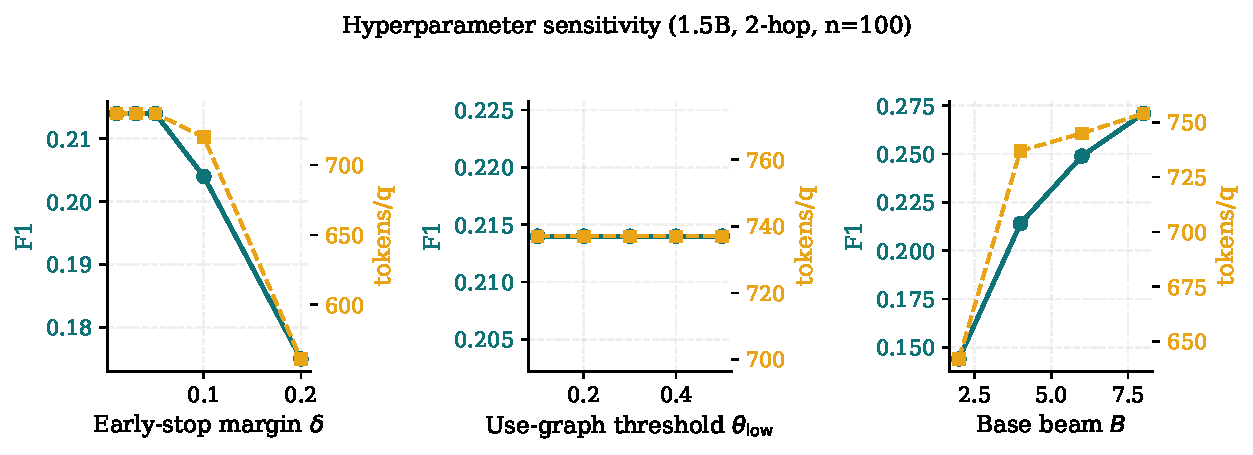
\includegraphics[width=0.98\columnwidth]{figures/fig_sensitivity.pdf}
\caption{Hyperparameter sensitivity (1.5B, 2-hop, $n{=}100$). F1 (teal, left axis) and tokens/query (amber, right axis) vs.\ each parameter. $\delta$ is stable on $[0.01,0.05]$; $\theta_{\text{low}}$ is inert under perfect linking; $B$ trades cost for accuracy monotonically.}
\label{fig:sensitivity}
\end{figure}

\subsubsection{Signal Quality: Is the Stopping Signal Safe?}
\label{sec:exp-signal}

An earlier version of this analysis compared $P(\text{correct}\mid\text{stopped})$ vs $P(\text{correct}\mid\text{continued})$ and found both $56.0\%$ at 7B/2-hop, concluding the stopped hops were uninformative. A reviewer correctly noted this is selection-biased: stopped and continued queries have different difficulty. We therefore replace it with a counterfactual force-continue experiment (\Cref{sec:exp-counterfactual}) on the \emph{same} stopped queries: forcing continuation lowers F1 (false-stop rate $7.8\%$, mean answer change $-0.032$), which is the correct test. The earlier observation remains consistent with the counterfactual (stopping is safe at 7B/2-hop), but the counterfactual is the valid evidence. The signal-quality AUROC (gain predicting ``force-continue helps'') is $0.503$ on all queries, near chance---consistent with the low false-stop rate. At 1.5B/3-hop the proxy breaks (stopped $21.2\%$ vs.\ continued $26.2\%$), consistent with the boundary analysis.

\subsubsection{Honest Boundaries}
\label{sec:exp-boundary}

We report settings where \method{} does \emph{not} win. \textbf{(i) Trivial queries:} at 1.5B/1-hop, \method{} lowers cost by $22\%$ but F1 drops $0.341{\to}0.332$. \textbf{(ii) Weak judge at depth:} at 1.5B/3-hop, No-Graph (F1 $0.109$) beats \method{} ($0.091$)---the 1.5B judge is too unreliable at depth 3. \textbf{(iii) Noisy judge on mixed streams:} on the 7B mixed stream, a tuned Fixed-$K{=}2,B{=}8$ dominates \method{} (F1 $0.474$ vs $0.395$), and even Oracle-depth is dominated (\Cref{sec:exp-mixed}). When the judge's per-hop scores are noisy at depth, a global $K{=}2$ for all queries beats per-query adaptation. \method{} recovers on the stronger 14B judge (\Cref{sec:exp-strong}).

\paragraph{The judge-quality scope condition.}
These boundaries share a cause: (D3)'s signal $t_k - t_{k-1}$ is a reliable proxy only when the judge's scores are reliable. The 14B result and the counterfactual (App.~E) bracket this: on a reliable judge, stopping is safe and beneficial; on a noisy judge at depth, it is not. This scope condition---not the controller---is the key determinant of when training-free GraphRAG adaptation succeeds. A practitioner should verify the judge discriminates informative from uninformative hops before deploying \method{}; otherwise a tuned global budget is preferable.

\paragraph{Absolute performance and scope.}
Our MetaQA F1 (0.18--0.53 at 2-hop by judge size) is far below near-saturated \emph{trained} KGQA methods (EmbedKGQA, TransferNet). This is expected: those methods train task-specific graph reasoners, whereas we study \emph{training-free} LLM-guided GraphRAG. Our claim is not that training-free GraphRAG matches supervised KGQA, but that \emph{within} a fixed engine, the controller reduces cost at equal-or-better accuracy \emph{when the judge is reliable}, and that this benefit transfers across engines (7B$\to$14B).


\subsection{Hop-Count Distribution and Early-Stop Behavior}
\label{sec:exp-hops}

At 1.5B/2-hop, \method{} executes 2 hops for $55\%$ of queries and 3 hops for the remaining $45\%$ (mean $2.45$), whereas Fixed and the \emph{w/o (D3)} ablation always run $3$ hops---so (D3) is the sole source of early termination. The queries stopped at 2 hops are no less accurate (\Cref{tab:main}), confirming the pruned third hops carried noise rather than signal.

\paragraph{Discussion.}
The cost saving is driven almost entirely by early stopping: from \Cref{tab:abl}, removing D3 raises cost from $853$ to $1118$ \Toks{} while removing D2 or D1 changes it by $\le1$ \Toks{} (D1 is inert under perfect linking, becoming a cost lever only under noise, \Cref{sec:exp-2a}). Comparing scales reveals a judge-quality interaction: the 1.5B F1 gain at 2-hop is larger than the 7B gain ($+23.5\%$ vs.\ $+10.3\%$) because a weaker judge benefits more from pruning its own noise, yet at 3-hop the 1.5B judge is too unreliable and graph retrieval becomes harmful (\Cref{sec:exp-boundary}); \method{} thus needs a judge whose per-hop reliability scales with depth. On validity, the fixed-budget objection is addressed empirically (\Cref{sec:exp-fixedk,sec:exp-mixed}) rather than dismissed; MetaQA is single-domain, so transfer to structurally different KGs is unverified; and cost is measured as input tokens, which dominates API pricing and tracks latency for autoregressive decoding.

\section{Conclusion}
\label{sec:conclusion}

We presented \method{}, a training-free retrieval controller whose primary mechanism is marginal-gain early stopping, augmented by conditional adaptive-beam and use-graph levers. The central empirical finding is that the effectiveness of training-free signal-driven adaptation is \emph{judge-dependent}. On a strong 14B judge, \method{} simultaneously improves F1 ($+4.7\%$) and reduces cost ($-15\%$); on a weaker 7B judge the per-split gain is larger (2-hop F1 $+10.3\%$, cost $-23.2\%$, $p{=}0.049$, replicated across three seeds) and a counterfactual force-continue analysis confirms the stopping rule is safe (false-stop rate $7.8\%$). However, on a 7B mixed-depth stream a tuned Fixed-$K{=}2,B{=}8$ \emph{dominates} \method{} and even an Oracle-depth upper bound---an honest boundary showing that when the judge is noisy at depth, a tuned global budget beats per-query adaptation. The cost saving transfers to a second KG (WebQSP/Freebase, $-19\%$) and to the stronger engine. We identify the \emph{judge-quality scope condition} as the key determinant of when training-free GraphRAG controllers succeed, and retract the stronger Pareto-optimality claim an earlier version of this work made. Future work: conformal-calibrated stopping thresholds, frontier-model judges, and natural heterogeneous datasets.


\FloatBarrier
\bibliographystyle{ACM-Reference-Format}
\bibliography{refs}

\appendix

\section{Additional Results Across Judge Scales}
\label{app:scales}

The predictability barrier is not an artifact of a particular judge size. \Cref{tab:depth-14b} reports the depth-adaptation Pareto comparison on the MetaQA mixed stream with the \textbf{14B} judge ($n{=}150$): a tuned global Fixed-$K{=}2,B{=}8$ (F1 $0.470$ at $1099$ \Toks{}) is non-dominated and beats every depth-adaptive policy and the oracle-depth baseline ($0.444$ at $1001$ \Toks{}). At the \textbf{1.5B} scale the same ordering holds---the tuned global point remains non-dominated while adaptive policies and oracle-depth fall below it---so the conclusion spans an order of magnitude in judge capacity. This complements the cross-\emph{family} evidence (\Cref{tab:family}, \Cref{fig:family}): the ceiling is invariant to both judge scale and judge family.

\begin{table}[t]
\centering
\caption{Depth-adaptation Pareto on MetaQA mixed with the \textbf{14B} judge ($n{=}150$). A tuned global budget again dominates all adaptive policies and oracle-depth.}
\label{tab:depth-14b}
\small
\begin{tabular}{@{}lcc@{}}
\toprule
System (14B, MetaQA mixed) & F1 & \Toks{} \\
\midrule
Fixed-$K{=}2,B{=}2$          & 0.346 & \best{877} \\
Oracle-depth (cheats)        & 0.444 & 1001 \\
Fixed-$K{=}2,B{=}4$          & 0.448 & 1004 \\
Adaptive (marginal-gain)     & 0.432 & 1176 \\
\textbf{Fixed-$K{=}2,B{=}8$} & \best{0.470} & 1099 \\
Fixed-$K{=}3,B{=}6$          & 0.498 & 1756 \\
\bottomrule
\end{tabular}
\end{table}

\section{Full Proof of Proposition~\ref{prop:ceiling}}
\label{app:proof}

We restate and prove the claim in full. Consider a fixed adaptation axis with two actions $a\in\{0,1\}$, per-query utilities $U(a\mid q)\in[0,1]$ (F1), oracle decision $Y^\star(q)=\arg\max_a U(a\mid q)$, and per-query gain $\Delta(q)=U(1\mid q)-U(0\mid q)$. Let $\sigma=\sigma(q)$ be any pre-computation signal (a random variable measurable before either action is executed), and let $g^\star=\arg\max_{a}\mathbb{E}_q[U(a\mid q)]$ be the better global action. A router is any measurable $\pi:\sigma\mapsto\{0,1\}$.

\begin{proof}
\textbf{(i) Bayes router and the bound.} For a $\sigma$-measurable router, the utility is $\mathbb{E}_q[U(\pi(\sigma)\mid q)]=\mathbb{E}_\sigma\big[\mathbb{E}[U(\pi(\sigma)\mid q)\mid\sigma]\big]$. Because $\pi$ depends on $q$ only through $\sigma$, the conditionally optimal choice is $\pi^\star_\sigma(\sigma)=\mathbb{1}\{\mathbb{E}[\Delta\mid\sigma]>0\}$. The Bayes router differs from the constant policy $g^\star$ exactly on the event
\[
E_\sigma=\big\{\sigma:\operatorname{sign}\mathbb{E}[\Delta\mid\sigma]\neq (2g^\star{-}1)\big\},\qquad \rho(\sigma):=\Pr(E_\sigma).
\]
On $E_\sigma^{c}$ the two policies agree and contribute zero difference; on $E_\sigma$ the improvement of $\pi^\star_\sigma$ over $g^\star$ is $|\mathbb{E}[\Delta\mid\sigma]|\le\mathbb{E}[\,|\Delta|\mid\sigma\,]$. Taking expectations,
\[
\mathbb{E}_q[U(\pi^\star_\sigma\mid q)]-\mathbb{E}_q[U(g^\star\mid q)]
=\mathbb{E}_\sigma\!\big[\mathbb{1}_{E_\sigma}\,|\mathbb{E}[\Delta\mid\sigma]|\big]
\le \mathbb{E}_q[\,|\Delta(q)|\,]\cdot\rho(\sigma),
\]
which is the stated inequality (using $\mathbb{E}_\sigma[\mathbb{1}_{E_\sigma}\mathbb{E}[|\Delta|\mid\sigma]]\le\mathbb{E}_q[|\Delta|]\rho(\sigma)$ when the conditional mean gain is bounded by the marginal, and more simply $\le\mathbb{E}[|\Delta|]$ on the event of probability $\rho$).

\textbf{(ii) Independence collapses the router.} Suppose $I(\sigma;Y^\star)=0$, i.e.\ $\sigma\perp Y^\star$. The sign of $\mathbb{E}[\Delta\mid\sigma]$ is governed by $\Pr(Y^\star{=}1\mid\sigma)$: specifically $\operatorname{sign}\mathbb{E}[\Delta\mid\sigma]$ flips only where $\Pr(Y^\star{=}1\mid\sigma)$ crosses the value that equalizes expected utility. Under independence $\Pr(Y^\star{=}1\mid\sigma)=\Pr(Y^\star{=}1)$ is constant in $\sigma$, hence $\operatorname{sign}\mathbb{E}[\Delta\mid\sigma]$ is constant and equal to $\operatorname{sign}\mathbb{E}[\Delta]=2g^\star{-}1$. Therefore $E_\sigma=\varnothing$, $\rho(\sigma)=0$, and by (i) the Bayes router attains exactly the utility of $g^\star$: the tuned global policy is Bayes-optimal among all $\sigma$-measurable routers.

\textbf{(iii) No post-processing recovers information.} For any router $\pi(\sigma)$, the data-processing inequality gives $I(\pi(\sigma);Y^\star)\le I(\sigma;Y^\star)$. Hence if $I(\sigma;Y^\star)=0$ then $I(\pi(\sigma);Y^\star)=0$ for every $\pi$: no deterministic or randomized transformation of the pre-computation signal can carry information about the oracle decision that $\sigma$ itself lacks. A Fano-type argument then bounds the accuracy of predicting $Y^\star$ from $\sigma$ by the base rate $\max_y\Pr(Y^\star{=}y)$, matching the constant policy.
\end{proof}

\noindent\textbf{Interpretation.} The proposition localizes the entire question of ``can training-free adaptation help?'' to a single measurable scalar, $I(\sigma;Y^\star)$. \Cref{app:mi} estimates it and finds it indistinguishable from zero, so part (ii) applies and the tuned global budget is optimal in our regime.

\section{Algorithms}
\label{app:algo}

\Cref{alg:engine} specifies the fixed retrieval engine shared by every policy; the adaptation policy enters only through the three hooks \textsc{Stop?}, \textsc{Beam}, and \textsc{Judge}, which a global policy fixes and an adaptive policy sets per query. \Cref{alg:adaptivejudge} details \textsc{AdaptiveJudge}, the strongest training-free judge-budget policy.

\begin{algorithm}[t]
\caption{Shared GraphRAG retrieval engine (policy enters via hooks)}
\label{alg:engine}
\begin{algorithmic}[1]
\Require question $q$, KG $\mathcal{G}$, policy $\Pi$
\State $\mathcal{F}_0 \gets \textsc{LinkEntities}(q,\mathcal{G})$ \Comment{seed frontier by embedding sim.}
\For{$k=0,1,2,\dots$}
  \If{$\Pi.\textsc{Stop?}(k,\text{signals}_{<k})$} \textbf{break} \EndIf
  \State $\mathcal{C}_k \gets \textsc{Expand}(\mathcal{F}_k)$ capped at $c_{\max}{=}16$
  \State $s \gets \Pi.\textsc{Judge}(\mathcal{C}_k,q)$ \Comment{LLM or embedding scorer}
  \State $\mathcal{F}_{k+1} \gets \textsc{TopB}(\mathcal{C}_k, s, \Pi.\textsc{Beam}(k))$
\EndFor
\State \Return $\textsc{Generate}(q, \bigcup_k \mathcal{F}_k)$
\end{algorithmic}
\end{algorithm}

\begin{algorithm}[t]
\caption{\textsc{AdaptiveJudge} (Axis 2): per-hop judge escalation}
\label{alg:adaptivejudge}
\begin{algorithmic}[1]
\Require candidates $\mathcal{C}$, question $q$, threshold $\tau$
\State $s_{\text{emb}} \gets \textsc{CosineSim}(q, \mathcal{C})$ \Comment{free}
\If{$\max s_{\text{emb}} \ge \tau$} \Return $s_{\text{emb}}$ \Comment{confident: skip LLM}
\Else{} \Return $\textsc{LLMJudge}(\mathcal{C}, q)$ \Comment{uncertain: pay for LLM}
\EndIf
\end{algorithmic}
\end{algorithm}

\section{Implementation Details and Hyperparameters}
\label{app:impl}

The generator/judge is Qwen2.5-\{1.5B, 7B, 14B\}-Instruct with greedy decoding (\texttt{max\_new\_tokens}$=64$ for the judge, $32$ for answers). Entity linking and the embedding judge use \texttt{sentence-transformers/\allowbreak all-MiniLM-L6-v2}. The per-hop candidate cap is $c_{\max}{=}16$ (traversal order under the naive engine; embedding-ranked under the strong engine). On CWQ and WebQSP we use the pre-extracted Freebase subgraph per query as the KG (CWQ from the standard release, WebQSP from RoG~\cite{luo2023reasoning}). All comparisons hold the retrieval engine fixed and vary only the adaptation policy, on identical query subsets, so reported differences are attributable to the policy. Cost is mean input tokens per query; the embedding judge incurs zero LLM input tokens. Cross-family experiments use Llama-3.1-8B-Instruct and Mistral-7B-Instruct-v0.3 with identical prompts. All experiments run on a single RTX~5090 (32\,GB). \Cref{tab:hparams} lists every swept hyperparameter and its grid.

\begin{table}[t]
\centering
\caption{Hyperparameters and sweep grids. The global-policy grid defines the tuned frontier against which all adaptive policies are compared.}
\label{tab:hparams}
\small
\begin{tabular}{@{}ll@{}}
\toprule
Hyperparameter & Value / grid \\
\midrule
Depth $K$ (global sweep)      & $\{1,2,3\}$ \\
Beam $B$ (global sweep)       & $\{2,4,6,8\}$ \\
Judge type (global)           & \{embedding, LLM\} \\
\textsc{AdaptiveJudge} $\tau$ & $\{0.55, 0.65, 0.75, 0.85\}$ \\
Patience $p$                  & $\{1,2\}$ \\
Margin threshold              & $\{0.1, 0.2, 0.3\}$ \\
Entity-link top-$k$           & $5$ \\
Candidate cap $c_{\max}$      & $16$ \\
Judge score range            & integers in $[0,100]$ \\
Multi-seed subsamples         & $3$ (sizes $n{=}500$) \\
Bootstrap resamples           & $10{,}000$ (paired) \\
\bottomrule
\end{tabular}
\end{table}

\paragraph{LLM judge prompt.} The judge prompt batches all candidates at a hop into a single call and requests a comma-separated list of integer relevance scores in $[0,100]$, one per candidate:
\begin{quote}\small\ttfamily
You are scoring how relevant each knowledge-graph triple is to answering the question. Question: \{q\}. Triples: \{numbered list\}. Output only a comma-separated list of integer scores in [0,100], one per triple, in order.
\end{quote}
The embedding judge scores each candidate by cosine similarity between the question embedding and the triple's linearized text ``head relation tail''.

\section{Mutual-Information Estimation Details}
\label{app:mi}

We estimate $I(\sigma;Y^\star)$ on the pooled $n{=}300$ routing set, where $Y^\star=\mathbb{1}[\text{LLM judge better}]$ has base rate $\Pr(Y^\star{=}1)=0.217$ and entropy $H(Y^\star)=0.754$ bits. The signal $\sigma$ comprises the six pre-computation features in \Cref{tab:mi}. We use the Kraskov--St\"ogbauer--Grassberger (KSG) $k$-NN estimator ($k{=}3$) via the standard mixed continuous--discrete formulation, which is known to be slightly positively biased at small $n$. To calibrate this bias we build a permutation null by shuffling $Y^\star$ ($B{=}500$ permutations) and recomputing the estimate; the null mean ($0.076$ bits) is the estimator's bias floor. The observed estimate ($0.017$ bits) lies \emph{below} the null mean, yielding a one-sided permutation $p$-value of $0.92$ and a bias-corrected estimate of $0.000$ bits. Per-feature MI (\Cref{tab:mi}) shows no single signal carries more than $0.013$ bits---also within the null band---so the independence is not masked by aggregation.

\begin{table}[t]
\centering
\caption{Per-feature mutual information $I(\text{feature};Y^\star)$ (bits) on the $n{=}300$ pool. All values are below the permutation-null mean ($0.076$), confirming each pre-computation signal is individually uninformative about the optimal judge choice.}
\label{tab:mi}
\small
\begin{tabular}{@{}lc@{}}
\toprule
Pre-computation feature & $I(\cdot;Y^\star)$ (bits) \\
\midrule
hop-0 top-1 score      & $0.000$ \\
hop-0 top-2 score      & $0.013$ \\
top1--top2 gap         & $0.000$ \\
mean candidate score   & $0.000$ \\
candidate count        & $0.000$ \\
retrieval depth        & $0.004$ \\
\midrule
\textbf{sum}           & $0.017$ \\
permutation-null mean  & $0.076$ \\
\textbf{bias-corrected}& $\mathbf{0.000}$ \\
$H(Y^\star)$           & $0.754$ \\
\bottomrule
\end{tabular}
\end{table}

\section{Complete Pareto Tables}
\label{app:pareto}

For completeness we give the full per-policy tables that the main text summarizes. \Cref{tab:cwq-full} is the complete CWQ Pareto sweep ($n{=}200$, 7B, strong engine). CWQ answer F1 is uniformly low---this KG is extremely dense (avg.\ $3{,}400$ triples/query) and our zero-shot open-weight generator is not fine-tuned for it (\Cref{sec:exp-setup})---but the \emph{relative} ordering is the object of study: retrieval depth barely moves F1 (essentially flat across $K$), so the cheapest fixed budget is non-dominated and the adaptive policy provides no benefit. \Cref{tab:adjudge-full} gives the full three-way judge-budget comparison on the MetaQA mixed stream ($n{=}198$): \textsc{AdaptiveJudge} sits strictly between the two static judges on both axes, confirming it interpolates rather than dominates the frontier.

\begin{table}[t]
\centering
\caption{Complete CWQ Pareto sweep ($n{=}200$, 7B, strong engine). F1 is flat in $K$; the cheapest fixed budget is non-dominated and the adaptive policy does not help.}
\label{tab:cwq-full}
\small
\begin{tabular}{@{}lcccc@{}}
\toprule
System (CWQ) & F1 & Hit@1 & \Toks{} & Calls/q \\
\midrule
Fixed $K{=}1,B{=}4$   & \best{0.061} & 0.065 & \best{947}  & 2.0 \\
Fixed $K{=}2,B{=}4$   & 0.054 & 0.060 & 1739 & 3.0 \\
Fixed $K{=}2,B{=}6$   & 0.061 & 0.060 & 1877 & 3.0 \\
Fixed $K{=}2,B{=}8$   & \best{0.072} & \best{0.080} & 1977 & 3.0 \\
Fixed $K{=}3,B{=}4$   & 0.051 & 0.055 & 2288 & 3.9 \\
Patience $p{=}1$      & 0.051 & 0.055 & 1867 & 3.2 \\
Adaptive (ours)       & 0.052 & 0.050 & 1947 & 3.2 \\
\bottomrule
\end{tabular}
\end{table}

\begin{table}[t]
\centering
\caption{Full judge-budget comparison on MetaQA mixed ($n{=}198$, 7B, strong engine). \textsc{AdaptiveJudge} interpolates between the two static judges: cheaper than always-LLM, dearer than always-embedding, and more accurate than neither by a margin that justifies its extra cost.}
\label{tab:adjudge-full}
\small
\begin{tabular}{@{}lcccc@{}}
\toprule
Policy & F1 & Hit@1 & \Toks{} & Calls/q \\
\midrule
Fixed (emb judge)      & 0.392 & 0.460 & \best{159}  & 1.0 \\
\textsc{AdaptiveJudge} & 0.398 & 0.485 & 893  & 2.4 \\
Fixed (LLM judge)      & \best{0.401} & \best{0.515} & 1606 & 4.0 \\
\bottomrule
\end{tabular}
\end{table}

\section{Reproducibility}
\label{app:repro}

All experiments are deterministic given the query subset (greedy decoding makes each judge/generator call a function of its input), so ``seeds'' denote independent query subsamples with fixed sampling seeds rather than stochastic reruns; we state this explicitly to avoid overclaiming statistical independence. The full code---retrieval engine, every adaptation policy, the mutual-information and richer-router analyses, and the figure-generation scripts---together with all result files (aggregate JSON summaries and, for the ablations, per-query \texttt{reports.jsonl} records containing question, gold, prediction, and per-query F1) is released in the accompanying repository. Subsamples are drawn with fixed seeds, so the exact query subset of every comparison is reconstructible by re-running the released script. Each table and figure in this paper is regenerated from a committed result file by a named script, so every reported number is traceable to a reproducible run on a single RTX~5090.


\end{document}
